
\documentclass{beamer}

\usetheme{Amsterdam}

\title[Short, Undeniable Signatures for Android 2.x]{Short, Undeniable Signatures for Android 2.x}
\subtitle{Master Semester Project}
\institute{EPFL}
\author[Sebastien Duc]{Sebastien Duc}
\date{June 15, 2012}

\usepackage{amsmath}
\usepackage{amssymb}
\usepackage{amsthm}
\usepackage{graphicx}
\usepackage{pstricks}

\useinnertheme{rectangles}

\newcommand{\legendre}[2]{\left(\frac{#1}{#2}\right)}

\newlength{\wideitemsep}
\setlength{\wideitemsep}{\itemsep}
\addtolength{\wideitemsep}{10pt}
\let\olditem\item
\renewcommand{\item}{\setlength{\itemsep}{\wideitemsep}\olditem}

\setlength\fboxsep{0pt}
\setlength\fboxrule{0.2pt}

\AtBeginSection[]
{
  \begin{frame}<beamer>
      \frametitle{Outline}
      \tableofcontents[currentsection,currentsubsection]
    \end{frame}
}

\AtBeginSubsection[]
{
  \begin{frame}<beamer>
      \frametitle{Outline}
      \tableofcontents[currentsection,currentsubsection]
    \end{frame}
}

\begin{document}
%------- Title ------
\begin{frame}
    \titlepage
\end{frame}
%------ Outline ----
\begin{frame}
    \frametitle{Outline}
    \tableofcontents[pausesections]
\end{frame}

%------- Introduction -------------
\section{Introduction}
\begin{frame}{Introduction (1)}
    \begin{itemize}
        \pause \item MOVA is an undeniable signature scheme.
        \pause \item It can achieve very small signatures.
        \pause \item Shortness of signatures is very convenient in mobile applications.
        \pause \item The aim of the project was to design an application for Android using MOVA.
    \end{itemize}
\end{frame}

\begin{frame}{Introduction (2)}
    \begin{itemize}
        \pause \item Today there exists a lot of application for classical signatures.
        \pause \item It is not the case for undeniable signatures (and MOVA).
        \pause \item We tried to find an application where undeniable signatures can bring something.
    \end{itemize}
\end{frame}


%------- MOVA ------------------
\section{Signature Schemes}

\subsection{Undeniable Signatures}

\begin{frame}{Specifications}
    \begin{itemize}
        \pause \item Undeniable Signatures are not universally verifiable. 
        \pause \item The verifier must run an interactive protocol with the signer 
    \end{itemize}
\end{frame}

\begin{frame}{Definition}
    Consider two participants $S$ and $V$.\\
    We define
    \begin{description}
        \pause\item[\bf Setup] $(k_p^S,k_s^S) \leftarrow \mathrm{Setup}^S(1^n)$ and 
        $(k_p^V,k_s^V) \leftarrow \mathrm{Setup}^V(1^n)$.
        \pause\item[\bf Sign] $\sigma \leftarrow \mathrm{Sign}(m,k_s^S)$ 
        \pause\item[\bf Confirm] Interactive protocol between $S$ and $V$ to confirm the validity of $(m,\sigma)$.
        \pause\item[\bf Deny] Interactive protocol between $S$ and $V$ to deny the validity of $(m,\sigma')$.
    \end{description}
\end{frame}

\subsection{MOVA}

\begin{frame}{MOVA Signature Scheme}
    \begin{itemize}
        \pause \item MOVA is a scheme for undeniable, short signatures. 
        \pause \item Provides batch verification.
        \pause \item Scheme based on group homomorphism.
    \end{itemize}
\end{frame}

\begin{frame}{Setup}
    Consider a pseudo-random generator $GenK$.
    \vspace{0.3cm}
    \begin{enumerate}
        \pause \item choose two groups $G,H$.
        \item choose a homomorphism $h:G\rightarrow H$
        \item Generate $Xkeys \leftarrow GenK(seedK)$, $Xkeys \in G^{Lkey}$.
        \item Compute $Ykeys = h^{Lkey}(Xkeys)$.
    \end{enumerate}
    \vspace{0.2cm}
    \pause Public key: $(G,H,|H|,seedK,Ykeys)$\\
    Secret key: $h$
\end{frame}

\begin{frame}{Signature}
    Consider a message $m\in\{0,1\}^*$ and the pseudo-random generator $GenS$.
    \vspace{0.5cm}
    \begin{enumerate}
        \pause \item Generate $Xsigs \leftarrow GenS(m)$, where $Xsigs \in G^{Lsig}$ 
        \item Compute $Ysigs = h^{Lsig}(Xsigs)$.
    \end{enumerate}
    \vspace{0.5cm}
    \pause Signature: $Ysigs$
\end{frame}

\begin{frame}{Group Interpolation}
    \begin{definition}
        We say the $S \subseteq G\times H$ interpolates in a group homomorphism if $\exists$ a homomorphism $h$ st.
        $h(x) = y$ $\forall (x,y) \in S$.
    \end{definition}

    Note: In MOVA we consider sets $S$ that interpolates in a unique group homomorphism.
\end{frame}

\begin{frame}{Verification}
    The verification is an interactive protocol between $S$ and $V$.\\
    \vspace{1cm}
    \pause The prover convinces the verifier that 
        \[\{(Xkey_i,Ykey_i)| i=1,...,Lkey\} \cup \{(Xsig_i,Ysig_i)|i=1,...,Lsig\}\]
    interpolates in a group homomorphism.
\end{frame}

\begin{frame}{Batch Verification}
    \begin{itemize}
        \pause \item Used to verify multiple signature.
        \pause \item Signatures must be issued from same key pair.
        \pause \item Verify all the signatures in only one protocol call.
    \end{itemize}
\end{frame}

%-------- The Application -------
\section{The Application}

\begin{frame}{Motivation}
    \begin{itemize}
        \pause \item The application is a University Contest
        \pause \item The concept is similar to the University Challenge in the UK, but using phones.
    \end{itemize}

\end{frame}

\subsection{Design}
\begin{frame}{Overview (1)}
    \begin{itemize}
            \pause\item Universities are providing quizzes to teams in other universities.
            \pause\item Teams win points by answering quizzes correctly and this increased the final score of their university. 
            \pause\item The university with the highest score wins the contest.
    \end{itemize}
\end{frame}

\begin{frame}{Overview (2)}
    \begin{itemize}
        \pause \item Quizzes are uniquely assigned to the teams.    
        \pause \item When subscribing, teams choose a password for future authentication.
        \pause \item Quizzes can contain normal or multiple choice questions.
        \pause \item Correction and scoring is done manually by the server manager.
    \end{itemize}
\end{frame}

\begin{frame}{Setup}
    Consider two universities $U_1$, $U_2$ and a team $T_i$ in university $U_2$.
    \begin{enumerate}
            \pause\item Server $S_1$ of $U_1$ provides quizzes to $T_i$ with a MOVA signature.
            \pause\item When filled-in, the quiz is sent to server $S_2$ of $U_2$.
            \pause\item $S_2$ signs it and send it back to $T_i$ with the signature.
            \pause\item $T_i$ can verify the signature and send it to $S_1$ with the signature.
    \end{enumerate}
\end{frame}

\begin{frame}
    \begin{minipage}[c]{0.4\textwidth}
            \centering
            Sending Quiz
            \begin{pspicture}(1,0)(4,5)
                \psellipse[fillcolor=gray!34,fillstyle=solid,linecolor=gray!34](1,2.5)(0.7,2)
                \psellipse[fillcolor=gray!34,fillstyle=solid,linecolor=gray!34](4,2.5)(0.7,2)
                \rput(1,4){\color{gray}$U_1$}
                \rput(4,4){\color{gray}$U_2$}
                \rput(1,3){$S_1$}
                \rput(4,3){$S_2$}
                \rput(4,1){$T_i$}
                \psline{->}(1.3,2.7)(3.7,1.3)
                \rput(2.5,2.5){$(Q,\sigma)$}
            \end{pspicture}
    \end{minipage}
    \hspace{1.5cm}
    \begin{minipage}[c]{0.4\textwidth}
            \centering
            Sending Quiz Back
            \begin{pspicture}(1,0)(4,5)
                \psellipse[fillcolor=gray!34,fillstyle=solid,linecolor=gray!34](1,2.5)(0.7,2)
                \psellipse[fillcolor=gray!34,fillstyle=solid,linecolor=gray!34](4,2.5)(0.7,2)
                \rput(1,4){\color{gray}$U_1$}
                \rput(4,4){\color{gray}$U_2$}
                \rput(1,3){$S_1$}
                \rput(4,3){$S_2$}
                \rput(4,1){$T_i$}
                \psline{->}(4.1,1.3)(4.1,2.7)
                \rput(4.3,2){\tiny $\tilde{Q}$}
                \psline{<-}(3.9,1.3)(3.9,2.7)
                \rput(3.5,2){\tiny $(\tilde{Q},\tilde{\sigma})$}
                \psline{<-}(1.3,2.7)(3.7,1.3)
                \rput(2.4,1.6){\tiny $(\tilde{Q},\tilde{\sigma})$}
            \end{pspicture}
    \end{minipage}
\end{frame}

\begin{frame}{Security}
    \begin{itemize}
        \pause \item Every signature is done with MOVA.
        \pause \item Quizzes are signed so that teams are ensured not to have a fake one.
        \pause \item Servers use batch verification. 
        \pause \item Teams are authenticated to their respective university server when sending the quizzes back.
        \pause \item Authentication is done using a simple challenge-response protocol.
    \end{itemize}
\end{frame}

\begin{frame}{Threat Model}
    An adversary could try the following
    \begin{itemize}
        \pause \item Forge fake quizzes. Hence the signature when sending quizzes. 
        \pause \item Fill in the quizzes of another team. Not possible by construction.
        \pause \item Modify the answers in a filled-in quiz. Hence the signature when sending back.
    \end{itemize}
\end{frame}

\begin{frame}{Implementation of MOVA}
    \begin{itemize}
        \pause \item $G = (\mathbb{Z}/n\mathbb{Z})^*$ where $n = pq$ is the product of two large primes.
        \pause \item $H = \{-1,1\}$.
        \pause \item The homomorphism can be either $\legendre{\cdot}{p}$ or $\legendre{\cdot}{q}$. 
    \end{itemize}
\end{frame}

\subsection{Application Result}

\begin{frame}{Client}
    \begin{columns}
        \column{.7\textwidth} % column designated by a command
        Android Application. It has three main activities.
        \begin{description} 
            \pause \item[\bf ChallengeActivity] To get the latest quiz. Answer to questions and send it back.
            \pause \item[\bf UniversityScoreActivity] To get the score of all participating universities. 
            \pause \item[\bf TeamScoreActivity] To get his team score and the results of the quizzes.
        \end{description}
        \column{.3\textwidth}
        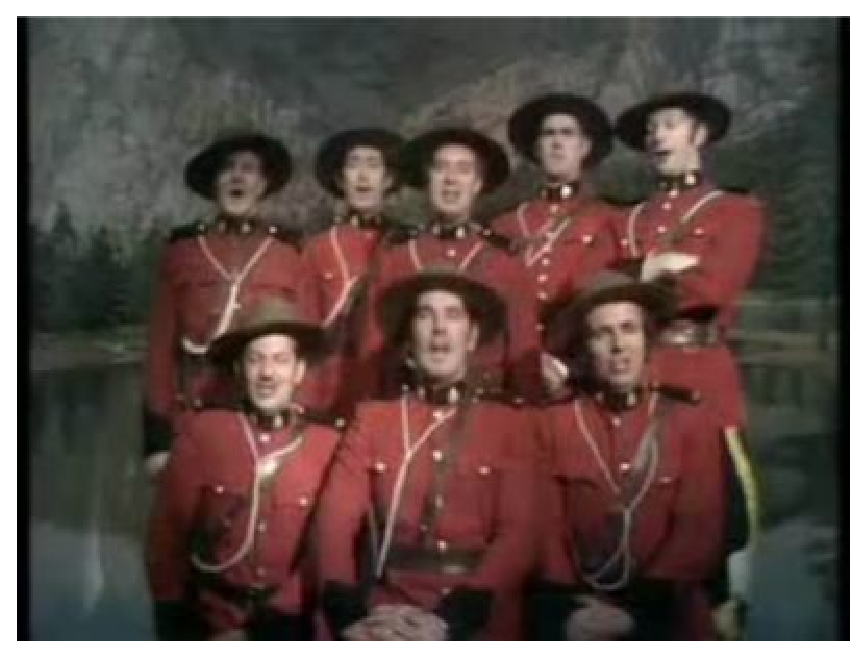
\includegraphics[width=\textwidth]{python1}
    \end{columns}
\end{frame}

\begin{frame}{Main Menu}
    \begin{center}
        \fbox{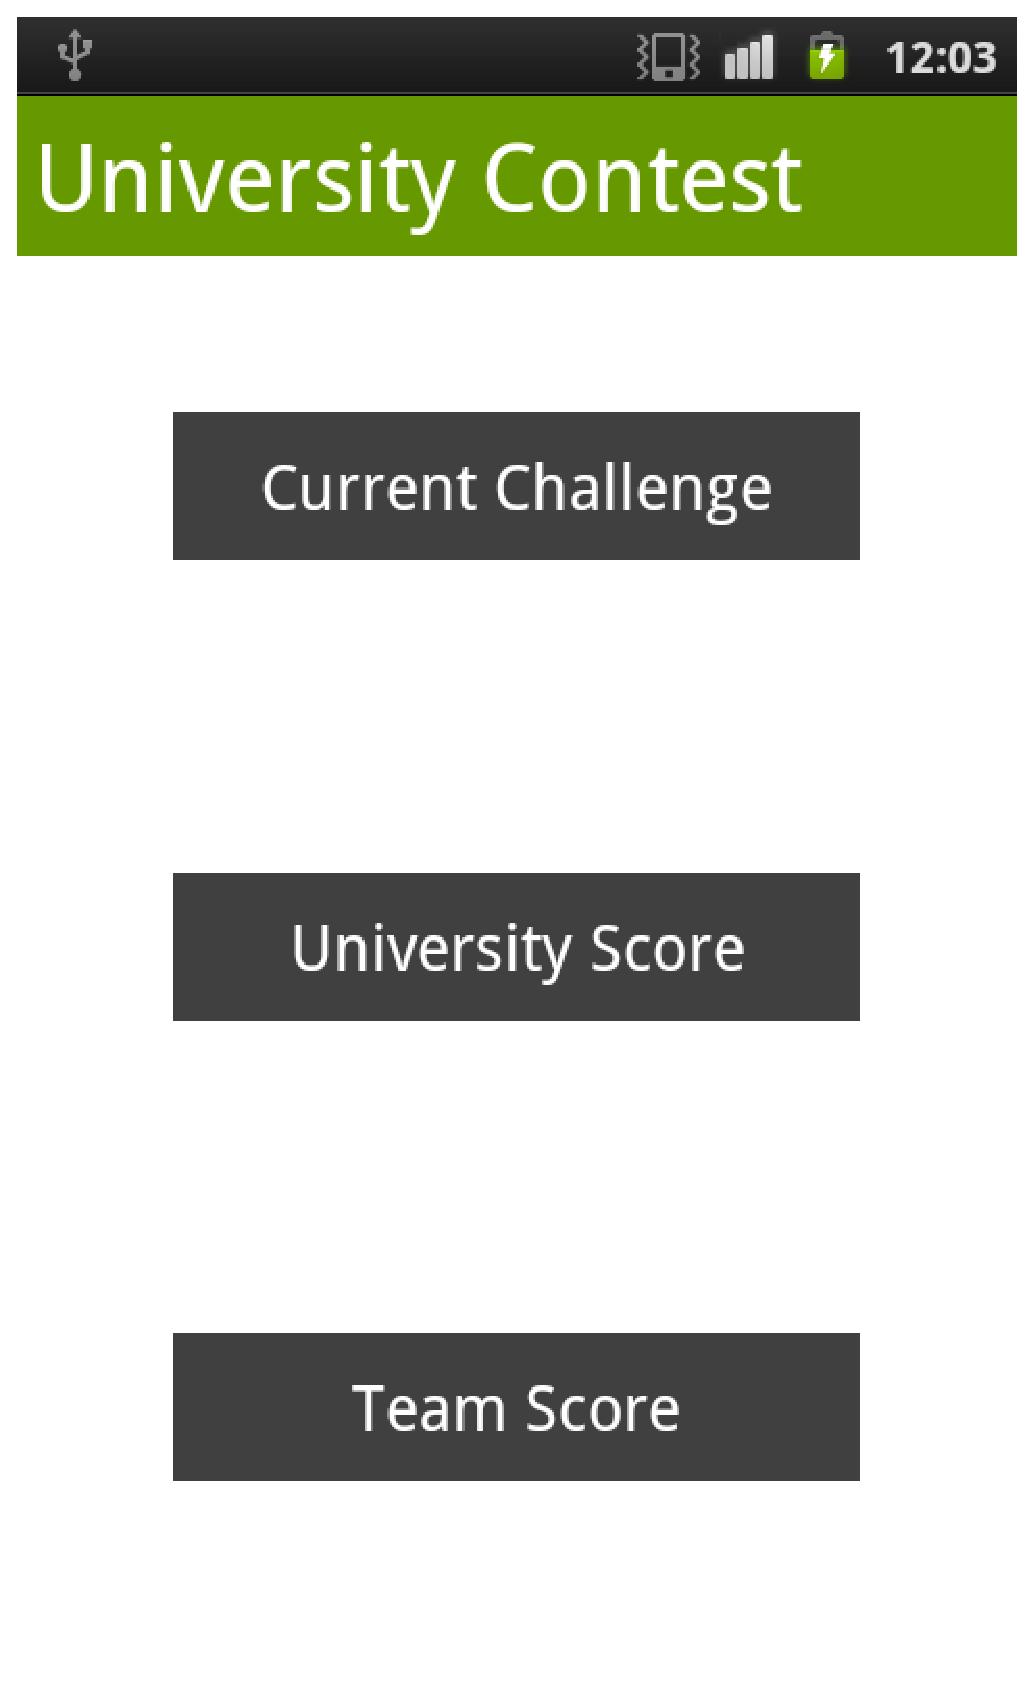
\includegraphics[width=0.3\textwidth]{../screenshots/unicontest_menu}}
    \end{center}
\end{frame}

\begin{frame}{ChallengeActivity}
    \begin{center}
        \fbox{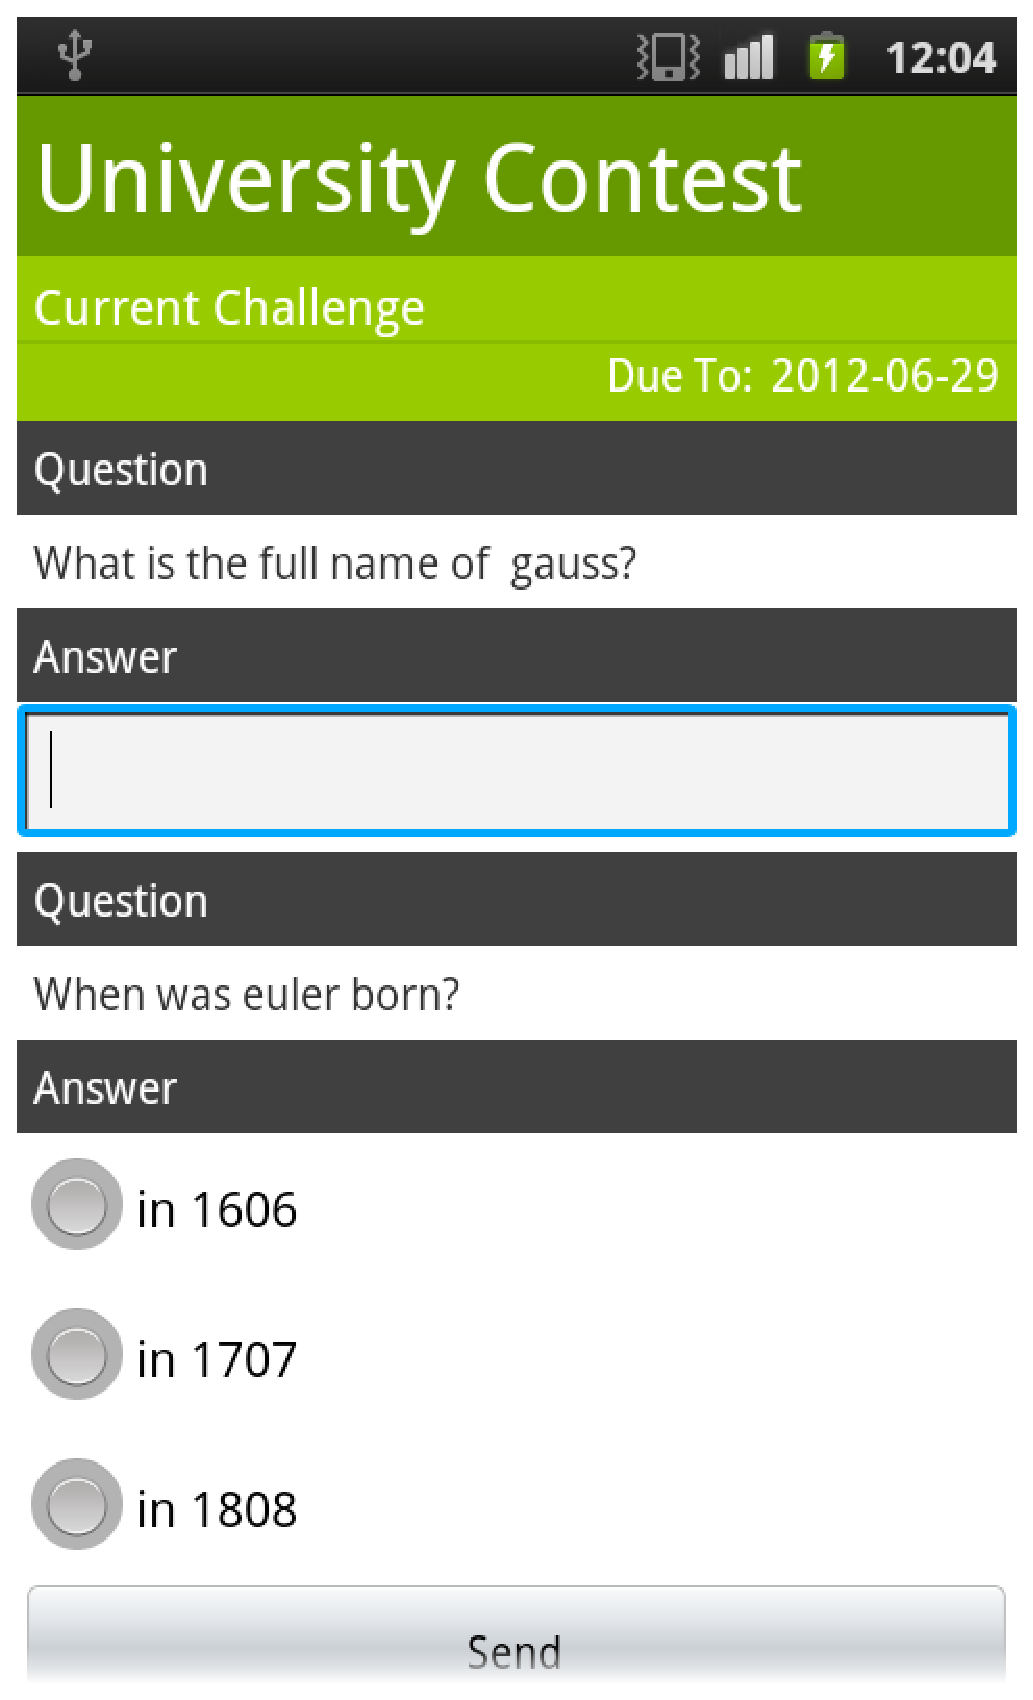
\includegraphics[width=0.3\textwidth]{../screenshots/unicontest_activity_quiz}}
    \end{center}
\end{frame}

\begin{frame}{UniversityScoreActivity}
    \begin{center}
        \fbox{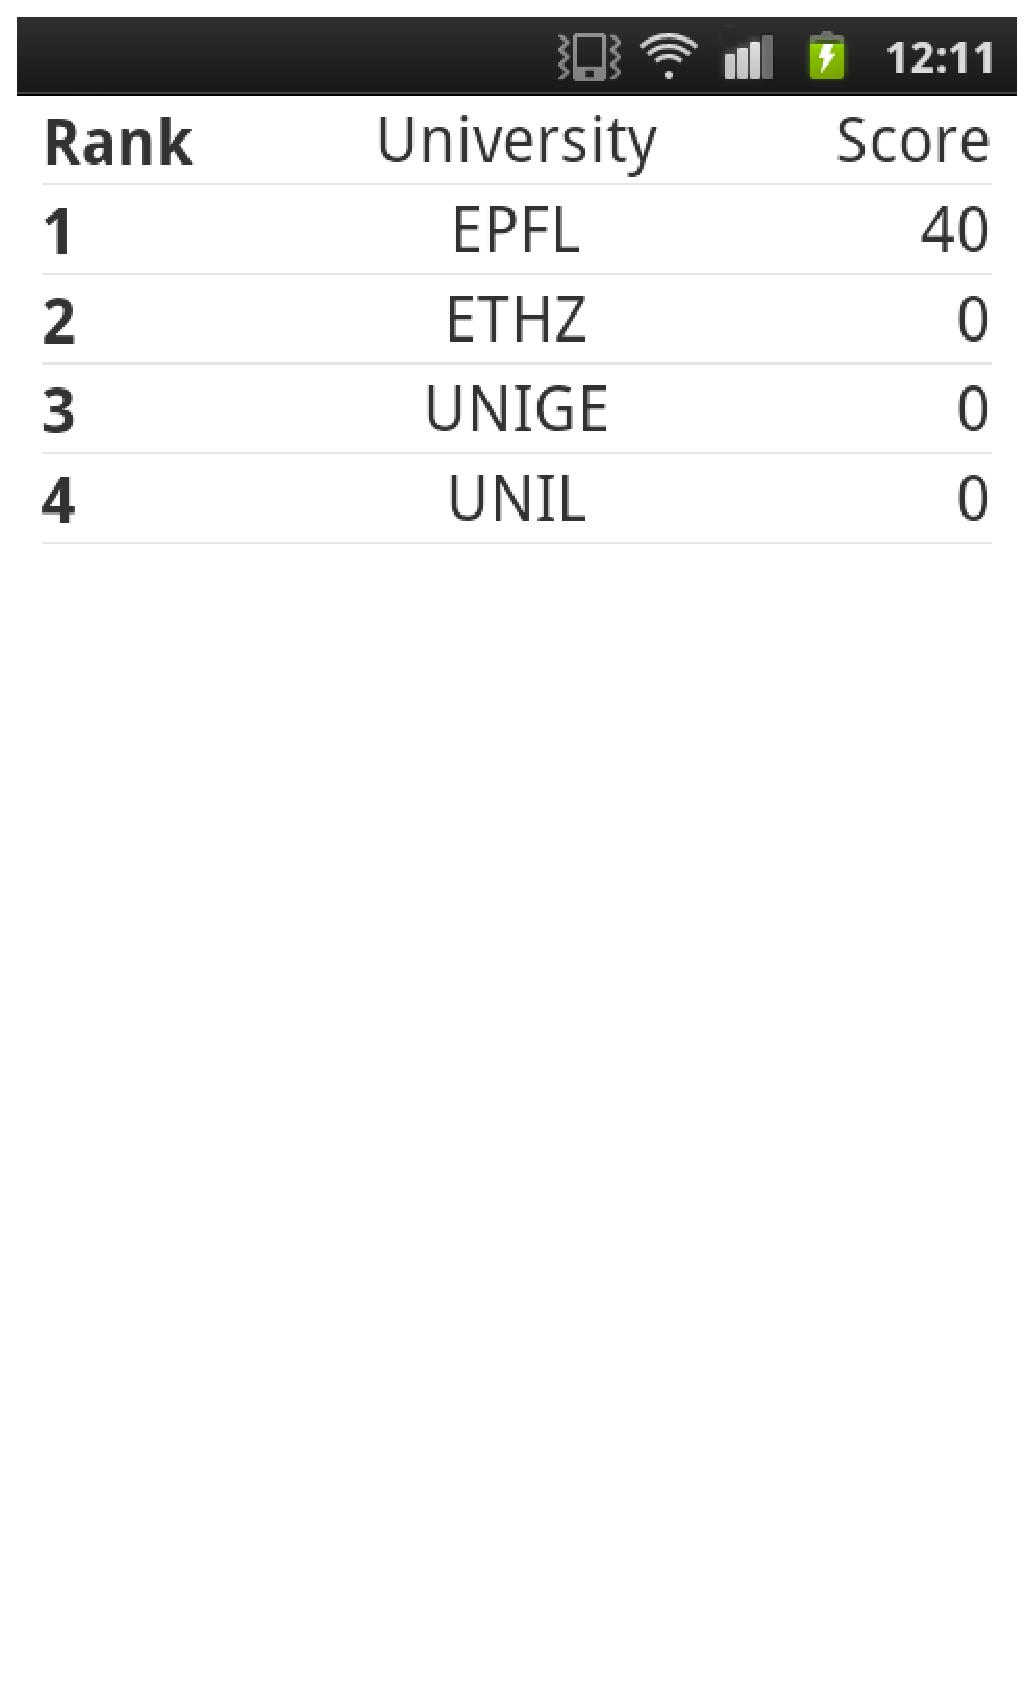
\includegraphics[width=0.3\textwidth]{../screenshots/unicontest_activity_uni}}
    \end{center}
\end{frame}

\begin{frame}{TeamScoreActivity}
    \begin{center}
        \fbox{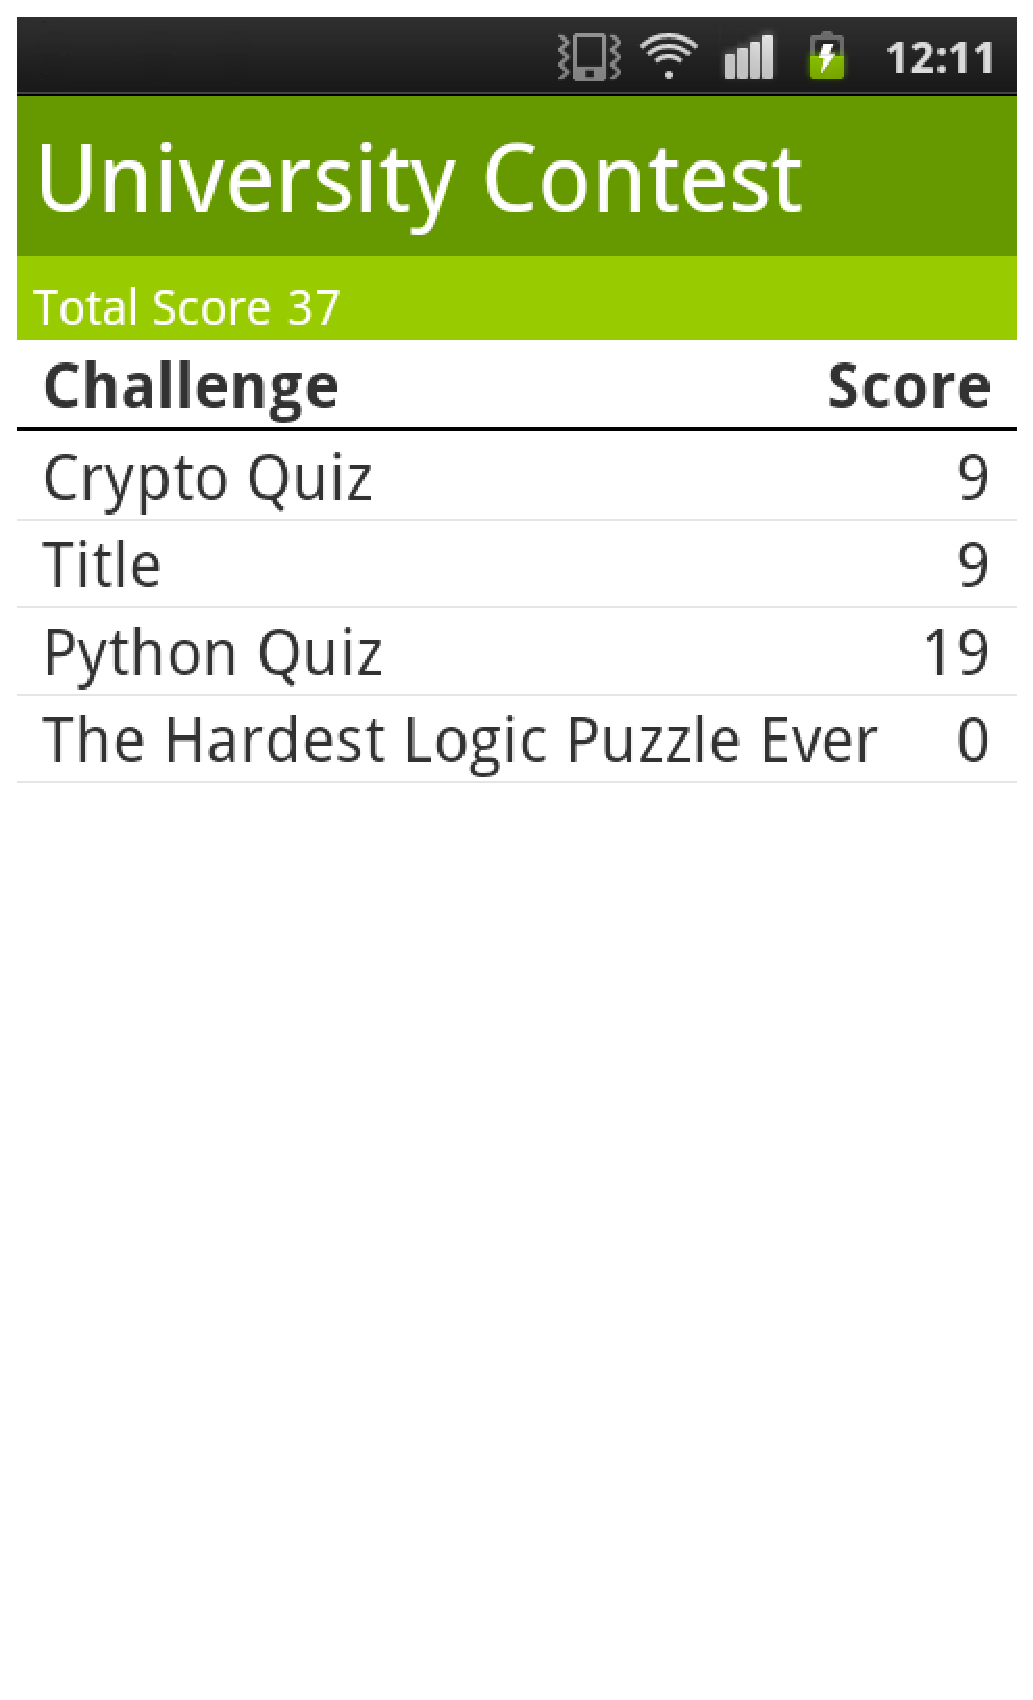
\includegraphics[width=0.3\textwidth]{../screenshots/unicontest_activity_team}}
        \hspace{2cm}
        \fbox{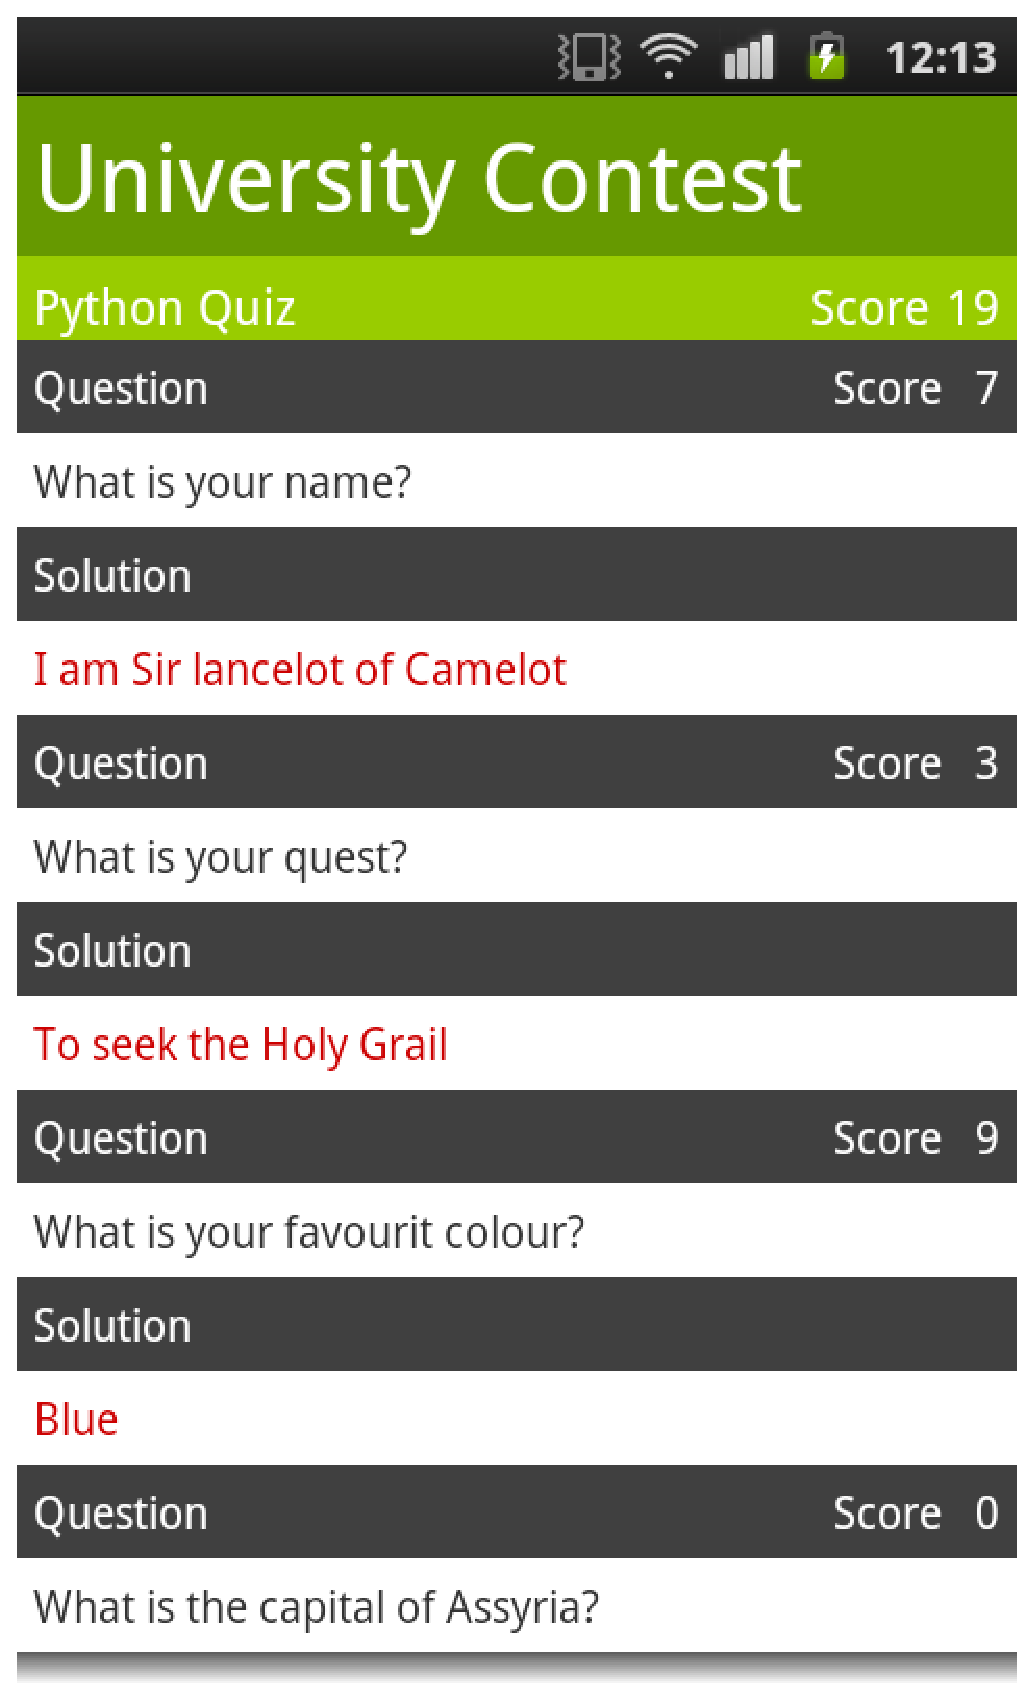
\includegraphics[width=0.3\textwidth]{../screenshots/unicontest_activity_quizresult}}
    \end{center}
\end{frame}

\begin{frame}{Server}
    Two Java applications and a MySQL database.
    \vspace{0.5cm}
    \begin{description}
    \pause \item[\bf Query Handler Process] A constantly alive thread listening to a specified port and answering to queries.
    \pause \item[\bf Server Manager] An application used to manage the server. Manage quizzes, teams and universities.
    \pause \item[\bf unicontest] The database consisting of three tables (team,challenge and university).
    \end{description}
\end{frame}

\begin{frame}{Challenge Manager}
    
\includegraphics[width =0.8\textwidth]{../screenshots/challenge_manager}
\end{frame}

%-------- Conclusion --------
\section{Conclusion}
\begin{frame}{Conclusion}
    \begin{itemize}
        \item We have designed an application for android using MOVA.
        \item MOVA serves such real-life mobile apps.: e.g., by its shortness  and by the batch verification. 
    \end{itemize}
    \vspace{1cm}
    \pause Future Work: Find other applications using MOVA which look a bit less artificial.
\end{frame}

\begin{frame}
     \begin{center}
         \Huge{Thanks for your attention !}
     \end{center}
\end{frame}


\end{document}
